\documentclass[a4paper, 11pt]{report}
\usepackage{blindtext}
\usepackage[T1]{fontenc}
\usepackage[utf8]{inputenc}
\usepackage{titlesec}
\usepackage{fancyhdr}
\usepackage{geometry}
\usepackage{fix-cm}
\usepackage[hidelinks]{hyperref}
\usepackage{graphicx}
\usepackage{titlesec}
\usepackage{graphicx}
\usepackage{subcaption}

\usepackage[english]{babel}

\geometry{ margin=30mm }
\counterwithin{subsection}{section}
\renewcommand\thesection{\arabic{section}.}
\renewcommand\thesubsection{\thesection\arabic{subsection}.}
\usepackage{tocloft}
\renewcommand{\cftchapleader}{\cftdotfill{\cftdotsep}}
\renewcommand{\cftsecleader}{\cftdotfill{\cftdotsep}}
\setlength{\cftsecindent}{2.2em}
\setlength{\cftsubsecindent}{4.2em}
\setlength{\cftsecnumwidth}{2em}
\setlength{\cftsubsecnumwidth}{2.5em}

\titlespacing\section{0pt}{12pt plus 4pt minus 2pt}{0pt plus 2pt minus 2pt}
\titlespacing\subsection{0pt}{12pt plus 4pt minus 2pt}{0pt plus 2pt minus 2pt}

\begin{document}
\titleformat{\section}
{\normalfont\fontsize{15}{0}\bfseries}{\thesection}{1em}{}
\titlespacing{\section}{0cm}{0.5cm}{0.15cm}
\titleformat{\subsection}
{\normalfont\fontsize{13}{0}\bfseries}{\thesubsection}{0.5em}{}
\titlespacing{\section}{0cm}{0.5cm}{0.15cm}

%=============================================================================

\pagenumbering{Alph}
\begin{titlepage}
\begin{flushright}

\includegraphics[width=4cm]{USyd}\\[2cm]
\end{flushright}
\center 
\textbf{\huge INFO1111: Computing 1A Professionalism}\\[0.75cm]
\textbf{\huge 2023 Semester 1}\\[2cm]
\textbf{\huge Self-Learning Report}\\[3cm]

\textbf{\huge Submission number: 1}\\[0.75cm]
\textbf{Github link: \href{https://github.com/oscarmoore1/Bubble.io}{Click here to visit my project}}\\[2cm]

{\large
\begin{tabular}{|p{0.35\textwidth}|p{0.55\textwidth}|}
	\hline
	{\bf Student name} & Oscar Moore\\
	{\bf Student ID} & 510549799\\
	{\bf Topic} & \textit{Swift}\\
	{\bf Levels already achieved} & ??\\
	{\bf Levels in this report} & A and B\\
	\hline
\end{tabular}
}
\thispagestyle{empty}
\end{titlepage}
\pagenumbering{arabic}


%=============================================================================

\tableofcontents

%=============================================================================


\newpage
\section{Level A: Initial Understanding}
\vspace{5mm}
\subsection{Level A Demonstration}
-Install and prepare an environment that supports swift\\
-Program and run a simple script\\
-Create a new model view in a separate script

\subsection{Learning Approach}
My approach to learning Swift mimics closely my approach to learning all programming languages. The first thing I did was first identify why I wanted to learn Swift. Prior to starting to study advanced computing at university, I had a clear goal of developing my own app. We live in a world that is heavily dominated by the apple ecosystem, hence, the logical next step was to choose a programming language that would work seamlessly with Apple’s frameworks and tools.\\
\\
The next step of my learning approach was understanding the basics of Swift. Understanding the basics of the language also included researching different environments that would support my project. Given that I was designing an app, Xcode would be the most appropriate platform to use, a necessity in the world of IOS app development.\\
\\
In order to further research the language itself, I heavily relied on the magic of Chatgpt. The system’s ability to scrape important information quickly and concisely, made the learning process seamless.


\subsection{Challenges and Difficulties}
Given the intuitive nature of SWIFT, I rarely ran into any technical difficulties (Other than a few thousand syntax errors). Having programmed in java and python before, Swift did not present a massive learning curve. With this being said, I ran into numerous challenges with regard to setting up the environment. Using the Xcode environment differed greatly from any IDE I had used before.\\
\\
My largest challenge was the lack of resources or materials available for learning in swift. While there are many resources available for Swift, they are less abundant than resources for more established languages like Java and Python. When I started programming my project, I ran into a bug that was unique to the new IOS 16 system, which was rarely covered on the apple developer website due to the novelty of the new apple software. This took the progress of my project to an abrupt halt until an anonymous respondee on the apple developer website answered my thread question.


\subsection{Learning Sources}
Learning Source - What source did you use? (Note: Include source details such as links to websites, videos etc.).	Contribution to Learning - How did the source contribute to your learning (i.e. what did you use the source for)?

\begin{tabular}{|p{0.45\textwidth}|p{0.45\textwidth}|}
	\hline
	Learning Source - What source did you use? (Note: Include source details such as links to websites, videos etc.). & Contribution to Learning - How did the source contribute to your learning (i.e. what did you use the source for)?\\
	\hline
Swift youtube video: \href{https://www.youtube.com/watch?v=6v4fmg9iRSU&t=87s&ab_channel=iOSAcademy}{click here} & Extremely helpful with regard to styling my swift project, also had good tips with how to organise class hierarchy.\\
	\hline
	Chatgpt & Helpful with debugging and solving syntax errors. Also gave me key functions that could be used based on use case prompts.\\
	\hline
	Apple developer & Very helpful for debugging code with errors that were not syntax.\\
	\hline
	Swift documentation: \href{https://www.swift.org/documentation/}{click here}  & Website used to access the swift documentation\\
	\hline
\end{tabular}

\subsection{Application artifacts}

My initial product proposal for this project was to create a messaging platform at a very basic level. The issue with this initial outlay was that in order to have users communicate through my app, I would have to integrate additional software tools such as Firebase (to store user information in a database). I deduced that it would be impossible to complete the project without collaboration with other tools. I will only cover the swift components of my project in this section of the report, however, I am aware that contributions from other languages/applications would be needed to complete the entirety of the project.\\
\\
My first objective was to create a landing page for the user. I added the Zeplin package to my project to further aid the design process. After a week of rigorous trial and error, I programmed the following:
\\
\\
Please proceed to the next page...

\begin{figure}
  \begin{subfigure}[h]{0.5\textwidth}
    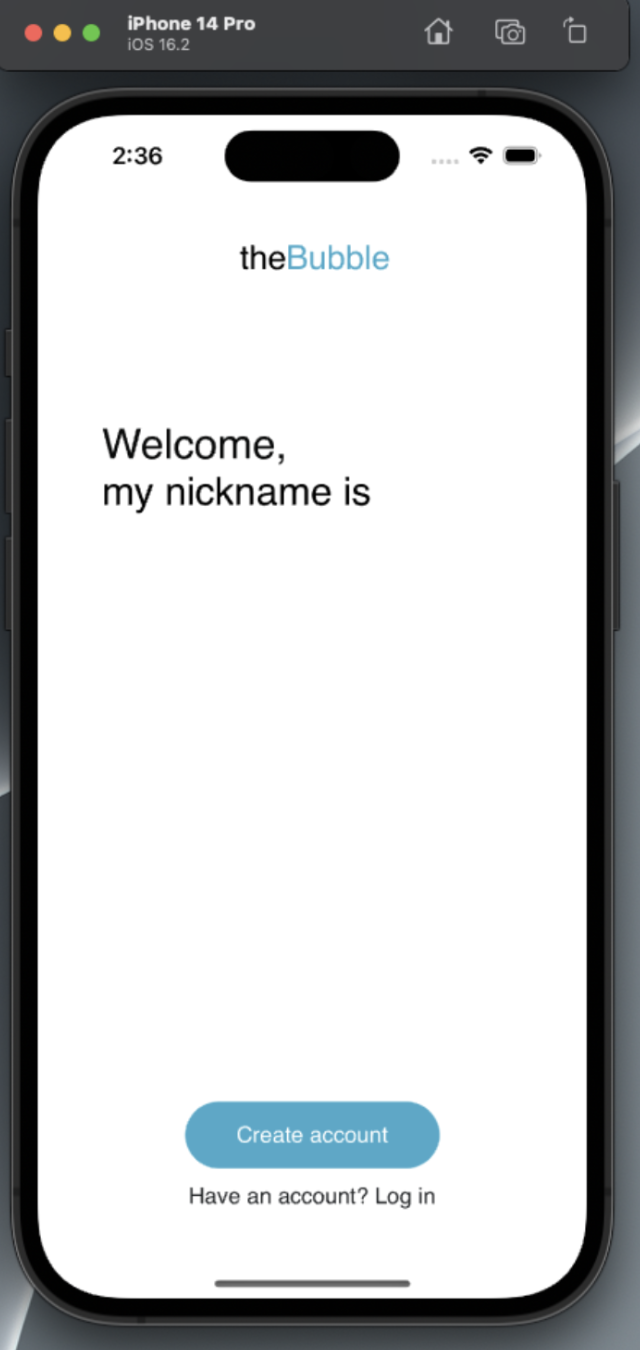
\includegraphics[width=\textwidth]{1.png}
    \caption{preview of landing page}
    \label{fig:image1}
  \end{subfigure}
  \hfill
  \begin{subfigure}[h]{0.7\textwidth}
    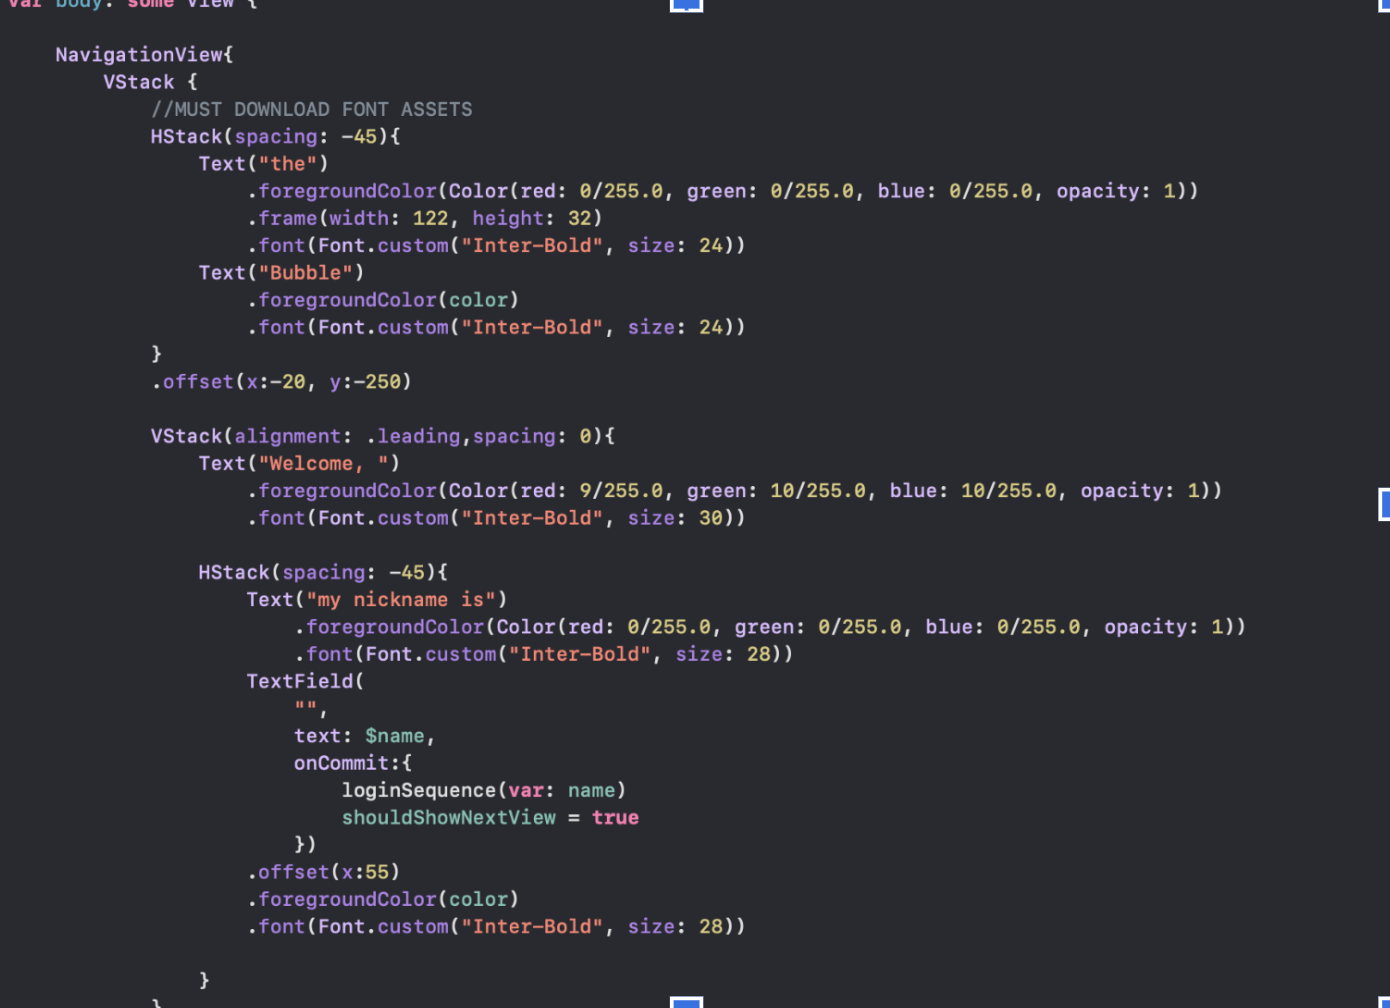
\includegraphics[width=\textwidth]{2.png}
    \caption{Sinpet of code for landing page}
    \label{fig:image2}
  \end{subfigure}
  \caption{The brunt of the information on the landing screen was included in a VStack as you can see above. This organized all my information vertically down the screen. In terms of the logic of the above code, there is very little. It is mostly formatting code so that it looks visually pleasing.\\}
  \label{fig:images}
\end{figure}


%=============================================================================
\newpage
The only challenging part above was managing the login sequence of the user. When the user writes in their username and presses the ‘enter’ key, the loginsequence() function is called.
\\
\begin{figure}[ht]
  \centering
  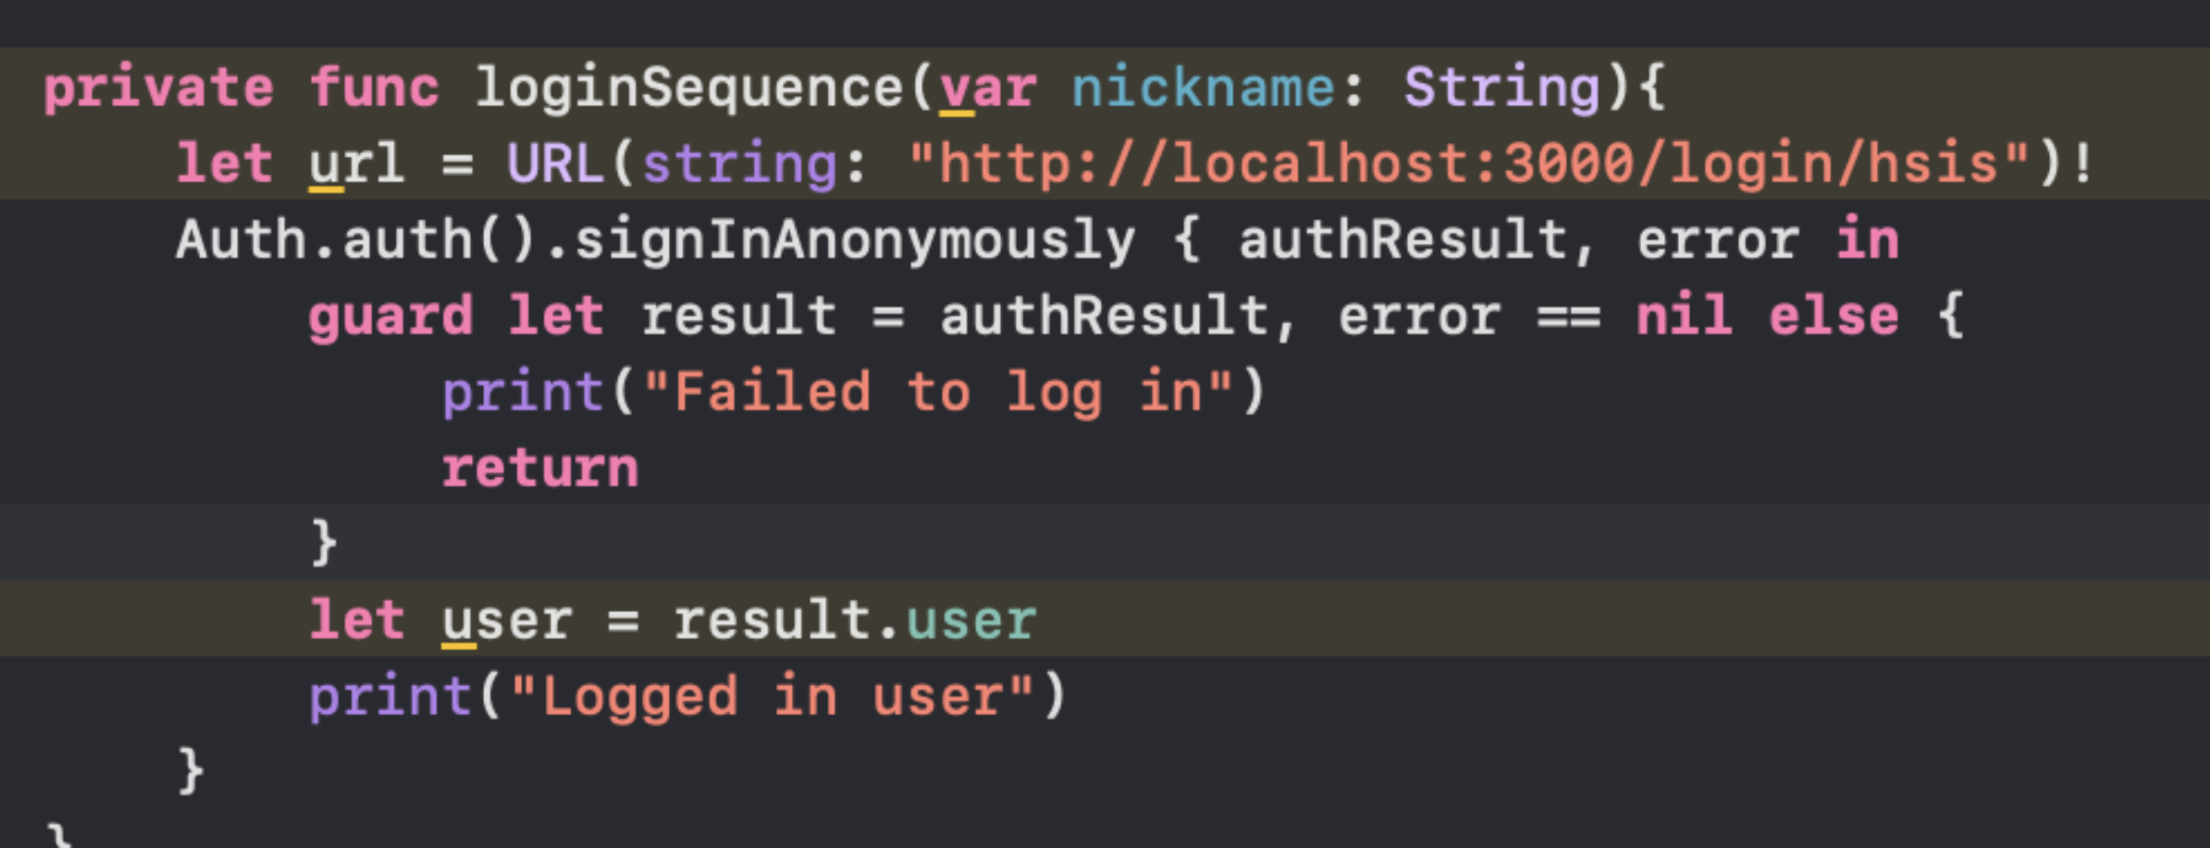
\includegraphics[width=0.8\textwidth]{3.png}
  \caption{Function code}
  \label{fig:example}
\end{figure}

This function basically registers the user into the database and authorises it to move to the next page. This is the first place that my program interacts with firebase, the user is given a unique identifier that is stored on the database. I decided to use the anonymous user authentication function that firebase provides since I wanted to avoid a long and tedious user registration process (The create account button on the display above was used in case the user wanted to save message history). If the login sequence is successful, the user is directed to the next swift page.

%=============================================================================

\newpage
\section{Level B: Basic Application}

Whilst level A is about doing something simple with the topic to just show that you have started to be able to use the tool or technology, level B is about doing something practical that might actually be useful.

\subsection{Level B Demonstration}

In order to make the project described above actually useful, I would have to draw up an appropriate use case.  I decided to slightly change the initial project outlay to include additional features that would make it a useful piece of software. \\
\\
Although a messaging app by itself would be highly useful, there are hundreds of much better alternatives already accessible. I decided to add an extra component to my app:\\
-The app would consider the location of the user\\
-I would have pre-defined group chats that could only\\ be accessed when the user was physically within the pre-defined radius.\\
-The app would suggest group chats that fall within the physical radius of the user.\\
\\
With the above requirements, the app would qualify as something that I would find useful to communicate with friends in my vicinity.



\subsection{Application artifacts}

Similar to the previous section, I will only provide artefacts that include code that I wrote in Swift since that is the topic I am self-learning.\\
The first step in providing the user with unique group chats based on location was by finding a way to pass information from a file into the Swift program. I decided to pass the parameters of the group chat (which I called bubbles in my app) using a JSON file, which my swift program read. The following screenshots include the JSON file with the necessary parameters for the ‘bubble’ and the config reader program I made to process this information.\\
\\
Please proceed to following page...

\begin{figure}
  \begin{subfigure}[h]{0.5\textwidth}
    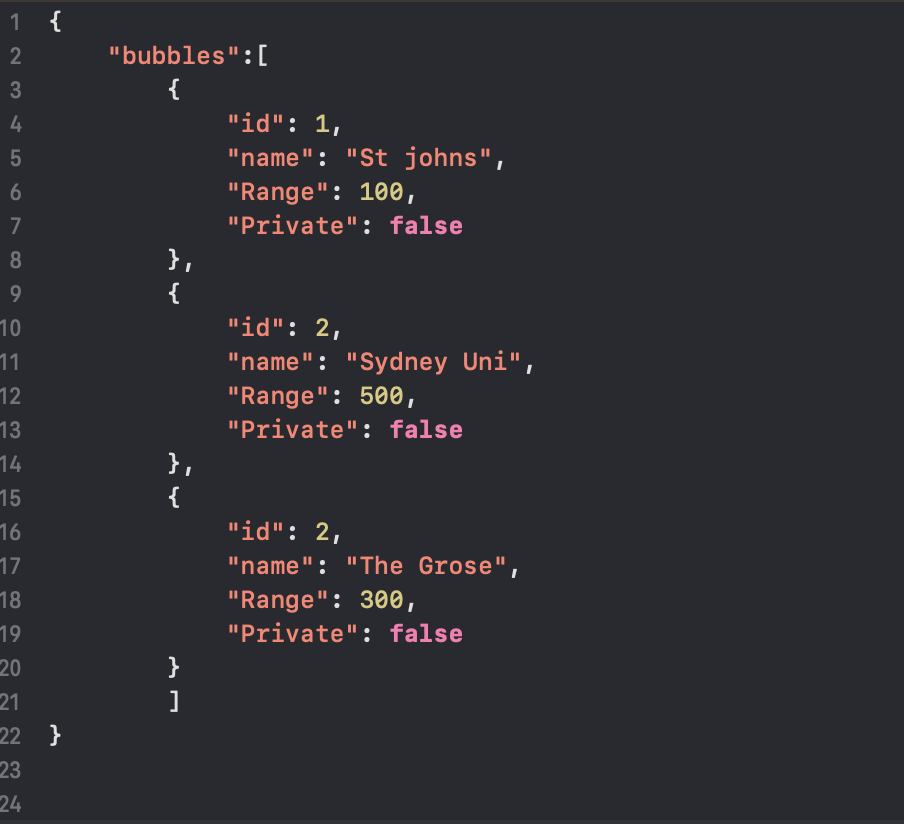
\includegraphics[width=\textwidth]{json.png}
    \caption{json example}
    \label{fig:image1}
  \end{subfigure}
  \hfill
  \begin{subfigure}[h]{0.6\textwidth}
    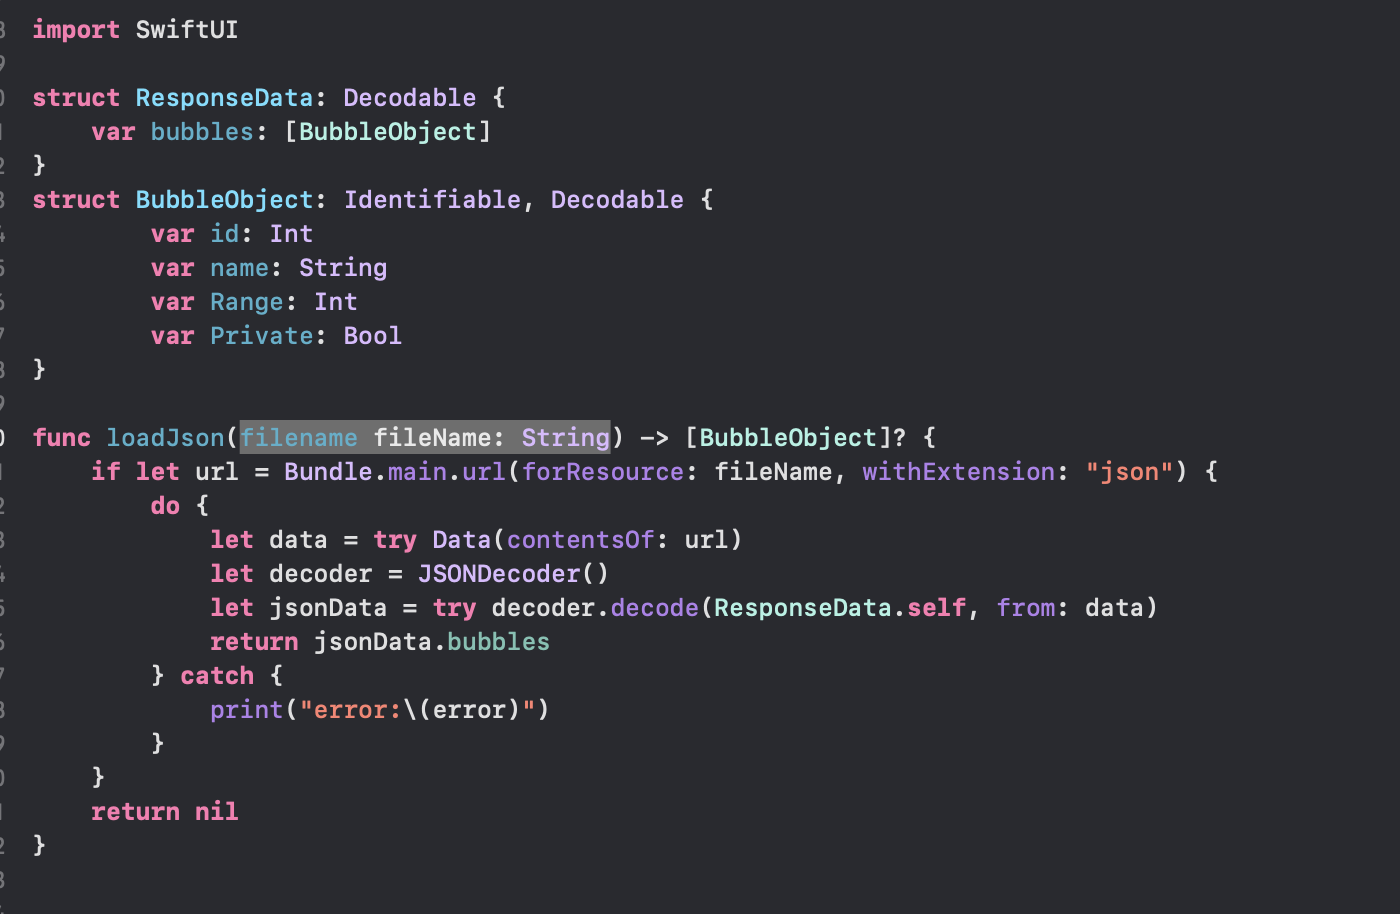
\includegraphics[width=\textwidth]{readjson.png}
    \caption{snipet of code used to read JSON}
    \label{fig:image2}
  \end{subfigure}
  \caption{
The way this works: the Swift file finds the JSON file in its local repository and passes it through a LoadJson() function. This function returns the bubble object in the correct format as defined by the structure in the code.\\
}

** What is my code doing and how it uses: variables, values, chaining classes, objects, namespaces?
The code above is creating an object that can read a JSON file. I do this so that I can retrieve information from a file and implement it in using my swift code. I make a bubble object class that will act as the group chat. The bubble object has variables: id (for bubble id), name (name of group chat) , range (range of bubble) and a boolean (to state whether the group chat is private or not). \\
I chain this class with the ResponseData class. The role of the response data class is that it creates an array of bubble objects, so that the user can have access to multiple group chats at once.\\
The namespace used here is the swiftUI module. The 'import' key word at the top of the code is used to bring the code defined in SwiftUi into my file. The library allows me to output previews of my code.**\\

\end{figure}

%=============================================================================
\newpage
\section{Level C: Deeper Understanding}

Level C focuses on showing that you have actually understood the tool or technology at a relatively advanced level. You will need to compare it to alternatives, identifying key strengths and weaknesses, and the areas where this tool is most effective. 

\subsection{Strengths}
What are the key strengths of the item you have learnt? (50-100 words)

I have learned many key strengths in Swift since undergoing my self-learning project.

I’ve learned about the simplicity of Swift. I’ve realised that Swift is an extremely intuitive and easy-to-learn language. This allows me to write clean, concise and readable code. This has also made it easier to understand and shortened the learning curve.

Its ability to be used for app development is also a large strength. Swift is specifically designed for app development, which means that it has been easy to find help and support online. Swift allows me to make powerful, high-performance apps that run seamlessly on Apple devices.

-Finally, the last strength I have learned is Swift’s speed. Swift has built-in optimization features that make the language incredibly fast. It uses modern-day compiler technology to generate highly optimized code, making it faster than other programming languages.


\subsection{Weaknesses}
What are the key weaknesses of the item you have learnt? (50-100 words)

One of the weaknesses of using Swift is it’s capability. Being a relatively new programming language, it is not fully backwards compatible with Obejctive-C, which can make it quite hard to integrate with legacy codebases.

It has limited support outside of the Apple ecosystem. Even though it is an extremely popular language for IOS and macOS development, it is not really used outside of the Apple ecosystem. Hence, it can limit the job opportunities available for a developer who specializes in swift.

Lastly, another weakness is that some tooling and libraries might not be as mature or feature-rich as those in other programming languages.


\subsection{Usefulness}
Describe one scenario under which you believe the topic you have learnt could be useful. (50-100 words)

A scenario under which I believe the topic I have selected could be useful is mobile development. Swift is a great language for mobile app development due to a few reasons. Firstly, it is the primary language for developing native IOS apps. Native apps have several advantages over web apps, these include better performance, access to native device features and better user experience. In addition to native app development, swift includes several features that help optimize app performance. These include automatic memory management which helps to reduce memory leaks and improve overall app performance. Swift also has built-in performance profiling tools that make it easier to optimise.

\subsection{Key Question 1}
Note: This question is in the table in the ‘Self Learning: List of Topics’ page on Canvas. (50-100 words)

There are several circumstances where Swift might be preferred over Python. Both programming languages have different strengths and weaknesses that make them better suited for different situations. The circumstances include the following:

Performance critical applications: Swift is generally faster since it is a compiled language. Compiled languages tend to be faster than interpreted languages like Python. In the circumstance that we need to write a performance-critical application such as a video game, Swift would be a better choice than Python.

Another circumstance where Swift would be preferred is if you need to develop any time of native IOS, macOS, watchOS, or TvOS applications. Since Swift is the primary language for developing native ios applications, it is preferred over other programming languages such as Python.


\subsection{Key Question 2}
Note: This question is in the table in the ‘Self Learning: List of Topics’ page on Canvas. (50-100 words)

Scenarios where using a closure might be more appropriate than a named function include:

If you need to write a simple function that will only be used once. Since it is only used only, we don’t have to name it and we can use a closure to keep our code concise. They can be useful when parsing functions as arguments for other functions.

Closures are more commonly used for sorting and filtering operations. This is because they are flexible and can be used to define custom sorting and filtering criteria for a variety of data types. Hence closure is more appropriate than named function in this case.



%=============================================================================

\newpage
\section{Level D: Evolution of skills}
\vspace{5mm}
\subsection{Level D Demonstration}

This is a short description of the application that you have developed. (50-100 words).
\textit{{\bf IMPORTANT:} You might wish to submit this as part of an earlier submission in order to obtain feedback as to whether this is likely to be acceptable for level D.}

\subsection{Application artifacts}

Include here a description of what you actually created (what does it do? How does it work? How did you create it?). Include any code or other related artefacts that you created (these should also be included in your github repository).

If you do include screengrabs to show what you have done then these should be annotated to explain what it is showing and what the application does.

\subsection{Alternative tools/technologies}
Identify 2 alternative tools/technologies that can be used instead of the one you studied for your topic. (e.g. if your topic was Python, then you might identify Java and Golang)
\subsection{Comparative Analysis}
Describe situations in which both your topic and each of the identified alternatives would be preferred over the others (100-200 words).



%=============================================================================

\newpage

\bibliographystyle{ieeetran}
\bibliography{main}

\end{document}
\end{report}
